
%\include{jiblm_cn}
\include{jiblm_djh} % My customized version
\usepackage{graphicx}
\usepackage{enumitem}
%%%% enumitem declarations
\newlist{problemparts}{enumerate}{1}
\setlist[problemparts,1]{label=(\alph*), itemsep=0pt, topsep=3pt}

\usepackage{thmtools}
%%%% thmtools declarations
\theoremstyle{definition}
\declaretheorem[numbered=no]{definition}
\declaretheorem[shaded={bgcolor=white}]{problem}
\declaretheorem[numbered=no]{theorem}

%%%% Useful abbreviations
\newcommand{\NN}{\mathbb{N}}
\newcommand{\RR}{\mathbb{R}}
\newcommand{\ZZ}{\mathbb{Z}}

%
%%%%%%%%%%%%%%%%%%%%% Annotation Environment Switch%%%%%%%%%%%%
%\StudentVersion
\InstructorVersion
%%%%%%%%%%%%%%%%%%%%% Annotation Environment Switch%%%%%%%%%%%%
%
\newcommand\blfootnote[1]{%
  \begingroup
  \renewcommand\thefootnote{}\footnote{#1}%
  \addtocounter{footnote}{-1}%
  \endgroup
}

\begin{document}
\large
\frontmatter
\title{Abstract Algebra I \& II}
\author{David J. Hunter$^1$ $<$ Margaret L. Morrow$^{2\dagger}$}
\affiliation{$^1$Westmont College \\ $^2$SUNY Plattsburgh}
\blfootnote{$^\dagger$The relation ``Hunter $<$ Morrow'' indicates that Chapters 1--5 of these notes were originally written by Margaret Morrow. David Hunter revised these chapters and added Chapters 6--13, and he takes full responsibility for this version of these notes.}
\maketitle

\tableofcontents

%%%%%%%%%%%%%%%%%%%%%%%%%%%%%%%%%%%%To the Instructor%%%%%%%%%%%%%%%%%%%%%%%%%%%%%%%%

\begin{annotation}
 \chapter{To the Instructor}

These notes provide an introduction to abstract algebra for advanced undergraduate mathematics majors. There should be enough material for a two-semester sequence. At Westmont College, most mathematics majors and some minors take first semester of this sequence, which (ambitiously) covers Chapters 1--9. These chapters contain a fairly standard treatment of groups, rings, and fields. Some of the more motivated mathematics majors, especially those destined for graduate school, will continue to the second semester, completing Chapters 10--13. The second semester includes some advanced group theory, including Sylow Theory, but its ultimate goal is to introduce students to Galois Theory.

This ultimate goal guides the selection of topics throughout these notes, beginning with the introductory activity. On the first day of class, students will discover how group operations can describe the symmetries of a polygon as permutations of the vertices. Analogously, by the end of the second semester, students will be using groups to describe automorphisms of splitting fields as permutations of the roots of a polynomial. It helps to keep the goal of the Galois correspondence in mind throughout both semesters, as it serves as a unifying theme.

At Westmont, enrollment for the first semester of this sequence is typically between 10 and 20, and second semester enrollment is much smaller. Regardless of class size, these notes are designed to be used with some form of the Moore method. Depending on the strength of the class, this method can be modified to provide additional support and scaffolding for students. I have found it very helpful to include the following components.
\begin{itemize}
    \item \textbf{Prework.} Before class, students should work independently on a selection of problems. I like to collect these preliminary solutions, either via online submissions or by running them through a scanner at the beginning of class. I grade these very leniently, giving full credit for what appears to be honest engagement with the problems. Currently, solutions to nearly every problem in every abstract algebra text can be found by searching the Internet, so lenient grading at this stage is essential. I tell students not to use any outside resources during the Prework stage, because I would rather see a half-right attempt at a problem of their own construction than a regurgitation of somebody else's solution.
    \item \textbf{Class Discussion.} During class, students will benefit by explaining their solutions, or lack thereof, to each other. These conversations can be encouraged in a variety of ways, using small-group discussion, class presentations, or a combination of the two. The goal of these discussions is to come to some consensus about a correct solution to each problem.
    \item \textbf{Postwork.} After class, students should be able to write up complete and correct solutions to every problem. These write-ups can be posted on a class wiki, maintained in a code repository, collected through a course management system, or kept in a journal. I carefully grade some subset of these assignments, where the subset size is determined by the size of the class.
\end{itemize}

Due to the abstract nature of the subject, it is important for instructors to provide some sort of regular framing and perspective on the material. Lectures will typically not be necessary, but students will appreciate hearing about why these techniques were developed and how these topics fit together.

The mathematical sophistication of the problems increases steadily throughout the sequence. Early on, students should be able to grapple with every detail of every proof. In later material, especially in the development of the Galois correspondence, some of the more difficult theoretical hurdles are given as theorems, with outlines, or ``sketches,'' of proofs. Often undergraduate treatments of Sylow and Galois theory simply state the main theorems and have students do calculations. While these notes do not require students to construct proofs of every theorem, they are designed to expose students to the theoretical development of the important results.

 Throughout the notes, you will notice superscripts at the end of some of the problems. These superscripts refer to endnotes in the last Chapter titled, ``Notes to the Instructor.''

\section*{Acknowledgements}

Chapters 1--5 were originally written by Margaret Morrow and published on \texttt{jiblm.org}. These chapters have been modified, but retain much of her original content. The remainder of these notes were heavily influenced by some of my favorite algebra texts, including the following.
\begin{itemize}
    \item \textit{A First Course in Abstract Algebra}, by John Fraleigh.
    \item \textit{A First Course in Abstract Algebra}, by Joseph Rotman.
    \item \textit{Contemporary Abstract Algebra}, by Joseph Gallian.
    \item \textit{Algebra}, by Thomas Hungerford.
    \item \textit{Galois Theory}, by Joseph Rotman.
\end{itemize}

\end{annotation}


%%%%%%%%%%%%%%%%%%%%%%%%%%%%%%%%%%%%To the Student%%%%%%%%%%%%%%%%%%%%%%%%%%%%%%%%

\chapter{To the Student}

Have you ever wondered how modern mathematics came to be? To what extent are the definitions and theorems that we find in the canonical textbooks the result of choices made by historical figures? Is there something intrinsic to the subject that forces modern mathematical theory down the path that it takes? Put another way, would Earthling mathematicians recognize the work of a community of mathematicians from a distant galaxy?

We can glean some insight into these questions by proceeding axiomatically: make as few assumptions and definitions as possible, and see where logical deduction leads. The material in these notes represents the consequences of some very low-level mathematical foundations: logic, sets, and the integers. These consequences have applications throughout pure and applied mathematics, and are part of the \textit{lingua franca} of the discipline.

Historically, much of this subject was motivated by the search for solutions to polynomial equations: are there analogs to the quadratic formula for polynomials of degree greater than~2? It is easy to believe that our hypothetical space-alien mathematical colleagues would also be interested in this question. Throughout this semester and the next (should you persevere), you will be guided through a series of deductive discoveries along the path that modern mathematicians have blazed. Whether this path is the only reasonable one will be yours to judge once you have completed the journey.

\begin{quote}
  \textit{That student is taught the best who is told the least.} ---R. L. Moore
\end{quote}

These notes (along with the sequel) give a comprehensive coverage of two semesters of advanced undergraduate or beginning graduate algebra. However, these notes contain mostly questions, and you must supply the answers. Your written accounts of your inquiry and our class discussions will produce a complete abstract algebra textbook of your own construction.

\mainmatter

\chapter*{Introductory Activity: Some Useful Examples}
\addcontentsline{toc}{chapter}{Introductory Activity}
\markboth{Introductory Activity}{Introductory Activity}

\textbf{Example I: Symmetries.}
\begin{annotation}
 \endnote{The introductory activity is designed to be done in groups on the first day of class, after a brief explanation of symmetries. Later material will refer to the examples that it introduces, so it is important not to skip it. You may wish to prepare the cut-out triangles and squares in advance. (Tip: provide only one triangle and one square per group, to encourage collaboration.) This activity also gives students a chance to solve some relatively concrete problems in a relaxed atmosphere. Ideally, each group should be able to send a representative to the board to record their answers. In addition to presenting these useful examples, the goal is to get students accustomed to sharing their work with the rest of the class. If time permits at the end of the group work, an informal whole-class discussion could look for patterns in the multiplication tables.}
\end{annotation}

We can think of a \textit{symmetry} of a plane figure as a rigid motion of the figure that results in the figure simply being repositioned on top of its original outline.

\textit{It is the final position of the figure that is important,} not the motion as such. For example, if we rotate the triangle below through $120^\circ$ or $480^\circ$, the triangle ends up in the same final position, so we do not think of these as distinct symmetries.

\begin{enumerate}
    \item Consider the symmetries of an equilateral triangle, as illustrated below. Each sketch shows the resulting position when the specified motion is applied to the triangle starting in the original position.
\begin{center}
    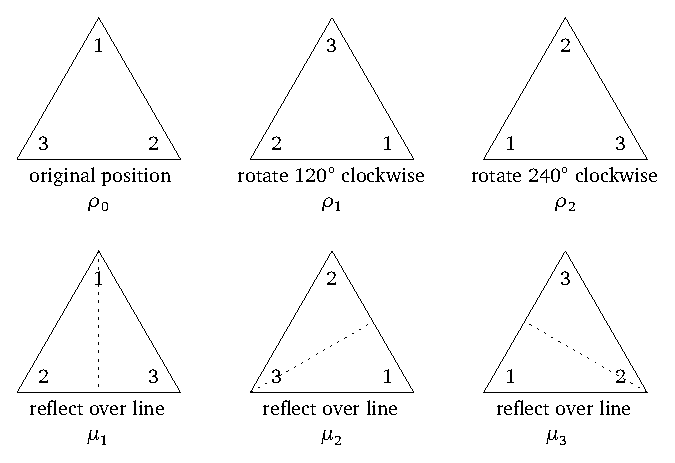
\includegraphics{wstriangles.eps}
\end{center}
    Cut an equilateral triangle out of a sheet of paper, and number the vertices 1, 2, and 3 as shown in the original position. Put the number of each vertex on the back of the triangle as well.

    We can apply one of the rigid motions, and then, \textit{continuing from the new position of the triangle,} apply another of the rigid motions. We can then record the overall effect as one of six symmetries listed above.

    For example if we first apply $\mu_1$, then (continuing from the resulting position) apply $\rho_1$ (a $120^\circ$ clockwise rotation) we end up with $\mu_2$. Using our usual function composition notation, we can write $\rho_1 \circ \mu_1 = \mu_2$.

    It is useful to write the results of all such combinations in table form, as shown below. We show the result of $\rho_1 \circ \mu_1$ in the row labeled $\rho_1$ and the column labeled $\mu_1$.

    \textbf{Important:} The convention is that we enter the result of $\rho_1 \circ \mu_1$ into the row corresponding to $\rho_1$ and the column corresponding to $\mu_1$, even though when we do these motions we first do the reflection $\mu_1$ and then the rotation $\rho_1$.

    \begin{center}
  \renewcommand{\arraystretch}{1.7}
    \begin{tabular}{|c||c|c|c|c|c|c|} \hline
        $\circ$ & $\rho_0$ & $\rho_1$ & $\rho_2$ & $\mu_1$ & $\mu_2$ & $\mu_3$ \\ \hline \hline
        $\rho_0$ & & & & & & \\ \hline
        $\rho_1$ & & & & & & \\ \hline
        $\rho_2$ & & & & & & \\ \hline
        $\mu_1$ & & & & & & \\ \hline
        $\mu_2$ & & & & & & \\ \hline
        $\mu_3$ & & & & & & \\ \hline
    \end{tabular}
    \end{center}

    Use the cut-out triangle to determine the result of all the compositions and complete the table. We will denote this collection of symmetries, together with composition, by $D_3$.

    \item You may have noticed that you can determine which symmetry was performed by looking at the labels of each vertex. Instead of representing rotations and reflections using Greek letters, it is often convenient to represent them using \textit{cycle notation.} For example, starting with the original position, the rotation $\rho_1$ moves vertex 1 to vertex 2, vertex 2 to vertex 3, and vertex 3 to vertex 1.
    \begin{center}
        
\includegraphics{d3cycles.eps}
    \end{center}
We can denote this rotation with the cycle $(1\; 2\; 3)$, which we read as ``1 goes to 2, 2 goes to 3, 3 goes to 1''. In cycle notation, each vertex moves to the one after it, and the last one wraps around to the first.

Complete the table below, giving the cycle that corresponds to each symmetry.
    \begin{center}
   \renewcommand{\arraystretch}{1.7}
    \begin{tabular}{|c|c|c|c|c|c|} \hline
         $\rho_0$ & $\rho_1$ & $\rho_2$ & $\mu_1$ & $\mu_2$ & $\mu_3$ \\ \hline
         $(1)$ & $(1\; 2\; 3)$ & $\phantom{(1\; 2\; 3)}$ & $(2\; 3)$ & $\phantom{(1\; 2\; 3)}$ & $\phantom{(1\; 2\; 3)}$ \\ \hline
    \end{tabular}
    \end{center}

\clearpage

    \item Develop similar tables for the symmetries of a square. We will use the notation $D_4$ for the symmetries of a square together with composition. Use the symbols indicated in the diagram below to denote the eight symmetries.
    \begin{center}
        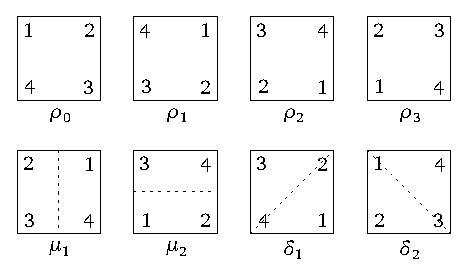
\includegraphics{wssquares.eps}
    \end{center}

    Using a cut-out square (or any other method), compute the compositions and fill out the following table.

    \begin{center}
  \renewcommand{\arraystretch}{1.7}
    \begin{tabular}{|c||c|c|c|c|c|c|c|c|} \hline
        $\circ$ & $\rho_0$ & $\rho_1$ & $\rho_2$ & $\rho_3$ & $\mu_1$ & $\mu_2$ & $\delta_1$ & $\delta_2$ \\ \hline \hline
        $\rho_0$ & & & & & & & &   \\ \hline
        $\rho_1$ & & & & & & & &  \\ \hline
        $\rho_2$ & & & & & & & &  \\ \hline
        $\rho_3$ & & & & & & & &  \\ \hline
        $\mu_1$ & & & & & &  & & \\ \hline
        $\mu_2$ & & & & & &  & & \\ \hline
        $\delta_1$ & & & & & &  & & \\ \hline
        $\delta_2$ & & & & & &  & & \\ \hline
    \end{tabular}
    \end{center}
    In addition, write each symmetry in cycle notation. (Notice that $\mu_1$ and $\mu_2$ need to be written as products of two disjoint cycles.)
    \begin{center}
   \renewcommand{\arraystretch}{1.7}
    \begin{tabular}{|c|c|c|c|c|c|c|c|} \hline
         $\rho_0$ & $\rho_1$ & $\rho_2$ & $\rho_3$ & $\mu_1$ & $\mu_2$ & $\delta_1$ & $\delta_2$ \\ \hline
         $(1)$ & $(1\; 2\; 3 \; 4)$ & $\phantom{(1\; 2\; 3\; 4)}$
         & $\phantom{(1\; 2\; 3\; 4)}$
         & $(1\; 2)( 3\; 4)$ & $\phantom{(1\; 2\; 3\; 4)}$ & $\phantom{(1\; 2\; 3\; 4)}$
         & $\phantom{(1\; 2\; 3\; 4)}$ \\ \hline
    \end{tabular}
    \end{center}
\end{enumerate}

\clearpage

\textbf{Example II: Clock arithmetic.} Consider the numbers on a clock, and imagine 0 in place of 12. (We will denote this set by $\mathbb{Z}_{12}$). So $\mathbb{Z}_{12} = \{0,1,2,3,4,5,6,7,8,9,10,11\}$.

We define ``addition modulo 12'' on this set as follows: for $a$ and $b$ in this set, $a + b \pmod{12}$ is the hour on the clock-face that is $b$ hours after $a$. For example, $9 + 5 = 2 \pmod{12}$, since 0 is 3 hours after 9, and we need an additional 2 hours after that.)

We can also define ``multiplication mod 12'' on $\mathbb{Z}_{12}$ by thinking of multiplication as repeated addition modulo 12. So for $a$ and $b$ in $\mathbb{Z}_{12}$, we think of $a\cdot b \pmod{12}$ as the result of adding $b$ to itself $a$ times, modulo 12. For example $3 \cdot 7 = 9 \pmod{12}$.

There is nothing special about 12 here; we can just as easily define addition and multiplication mod $n$ on the set $\{0,1,2,...,n-1\}$ for any fixed positive integer $n$. Simply imagine a clock-face with the numbers $\{0,1,2,...,n-1\}$ in place of $\{0,1,2,3,4,5,6,7,8,9,10,11\}$, and for $a$ and $b$ in this set, define $a+b \pmod{2}$ to be the hour on this clock-face that is $b$ hours after~$a$. Define $a\cdot b \pmod{n}$ to be the result of adding $b$ to itself $a$ times, modulo $n$.

We can draw up tables for these operations, just as we did for symmetries.
\begin{enumerate}
    \item Consider $\mathbb{Z}_5 = \{0,1,2,3,4\}$ Draw up a table for addition mod 5, and a separate table for multiplication mod 5.
    \begin{center}
  \renewcommand{\arraystretch}{1.7}
    \begin{tabular}{|c||c|c|c|c|c|} \hline
        $+$ & $0$ & $1$ & $2$ & $3$ & $4$  \\ \hline \hline
        $0$ & $\phantom{00}$ & $\phantom{00}$ & $\phantom{00}$ & $\phantom{00}$ & $\phantom{00}$ \\ \hline
        $1$ & & & & &  \\ \hline
        $2$ & & & & &  \\ \hline
        $3$ & & & & &  \\ \hline
        $4$ & & & & &  \\ \hline
    \end{tabular}
    \hspace{0.5in}
    \begin{tabular}{|c||c|c|c|c|c|c|} \hline
        $\cdot$ & $0$ & $1$ & $2$ & $3$ & $4$  \\ \hline \hline
        $0$ & $\phantom{00}$ & $\phantom{00}$ & $\phantom{00}$ & $\phantom{00}$ & $\phantom{00}$ \\ \hline
        $1$ & & & & &  \\ \hline
        $2$ & & & & &  \\ \hline
        $3$ & & & & &  \\ \hline
        $4$ & & & & &  \\ \hline
    \end{tabular}
    \end{center}
    \item Consider $\mathbb{Z}_6 = \{0,1,2,3,4,5\}$ Draw up a table for addition mod 6, and a separate table for multiplication mod 6.
    \begin{center}
  \renewcommand{\arraystretch}{1.7}
    \begin{tabular}{|c||c|c|c|c|c|c|} \hline
        $+$ & $0$ & $1$ & $2$ & $3$ & $4$ & $5$ \\ \hline \hline
        $0$ & $\phantom{00}$ & $\phantom{00}$ & $\phantom{00}$ & $\phantom{00}$ & $\phantom{00}$ & $\phantom{00}$ \\ \hline
        $1$ & & & & & & \\ \hline
        $2$ & & & & & & \\ \hline
        $3$ & & & & & & \\ \hline
        $4$ & & & & & & \\ \hline
        $5$ & & & & & & \\ \hline
    \end{tabular}
    \hspace{0.5in}
    \begin{tabular}{|c||c|c|c|c|c|c|} \hline
        $\cdot$ & $0$ & $1$ & $2$ & $3$ & $4$ & $5$ \\ \hline \hline
        $0$ & $\phantom{00}$ & $\phantom{00}$ & $\phantom{00}$ & $\phantom{00}$ & $\phantom{00}$ & $\phantom{00}$ \\ \hline
        $1$ & & & & & & \\ \hline
        $2$ & & & & & & \\ \hline
        $3$ & & & & & & \\ \hline
        $4$ & & & & & & \\ \hline
        $5$ & & & & & & \\ \hline
    \end{tabular}
    \end{center}
\end{enumerate}

\chapter{Introduction to Groups}

In this course, we stipulate the meanings of the terms and symbols using \textit{definitions}. When faced with a new definition, try to understand it by thinking of examples that satisfy the conditions of the definition.  It also helps to try to come up with ``non-examples,'' meaning entities closely related to the defined concept, but that do not conform precisely to the definition.

\begin{definition}
    A \textbf{binary operation} \(*\) on a set \(A\) is a function \(A \times A \rightarrow A\), where \((a,b) \mapsto a*b\).  In other words, a binary operation inputs two elements \(a\), \(b\) of the set \(A\), and outputs a well-defined element \(a * b\) of the set \(A\).
\end{definition}

\begin{problem}\label{prob:binops}
Which of the following are binary operations on the specified set? If not, explain why not.
\begin{problemparts}
  \item Addition on \(\mathbb{Z}\), the set of integers.
  \item Subtraction on \(\mathbb{Z}\), the set of integers.
  \item Subtraction on \(\mathbb{N}\), the set \(\{1,2,3,\ldots\}\) of natural numbers.
  \item Division on \(\mathbb{R}\), the set of real numbers.
  \item Division on \(\mathbb{Z}\setminus \{0\}\).
  \item Composition on \(D_4\), the symmetries of the square.
  \item Composition on the set of rotations in \(D_4\).
  \item Multiplication modulo 6 on \(\mathbb{Z}_6\).
\end{problemparts}
\end{problem}

\begin{definition}
A binary operation is \textbf{associative} if \((a * b)*c = a*(b*c)\) for all \(a,b,c \in A\).  An element \(e\) is said to be an \textbf{identity} for~\(*\) if \(a*e = e*a = a\) for all \(a \in A\).
An element \(b\) is an \textbf{inverse} of the element \(a\) if \(a * b = b * a = e\).
\end{definition}

\begin{problem}
Refer back to those operations in Problem~\ref{prob:binops} that were binary operations.
Do the following for each of these binary operations.
\begin{problemparts}
  \item Determine whether the operation is associative, and if not, prove that the operation is not associative.
  \item State whether there is an identity for the operation, and if so, identify it.
  \item If there is an identity for the operation, determine which elements (if any) have inverses.
\end{problemparts}
\end{problem}

\clearpage % so the definition and problem are together

\begin{definition}
    A binary operation is \textbf{commutative} if \(a * b = b * a\) for all \(a,b \in A\).
\end{definition}

\begin{problem}
Determine which of the binary operations in Problem~\ref{prob:binops} are commutative, and if not, provide proof that the operation is not commutative.
\end{problem}

\begin{problem}
Prove that if a binary operation \(*\) on a set \(A\) has an identity element, then that identity element is unique.
\end{problem}

\begin{definition}
A \textbf{group} is a set \(G\) together with a binary operation \(*\) on \(G\) satisfying the following:
\begin{enumerate}[itemsep=0pt, topsep=3pt]
  \item The operation \(*\) is associative.
  \item There is an element in \(G\) which is an identity for \(*\).
  \item Every element in \(G\) has an inverse with respect to \(*\) in \(G\).
\end{enumerate}
We denote the group by \(\langle G, * \rangle\). We refer to the set \(G\) as the \textbf{underlying set} of the group \(\langle G, * \rangle\). (However if the specific operation is clear from the context, or is not important in the context, we sometimes simply write \(G\) instead of \(\langle G, * \rangle\) for the group, and speak of ``the group \(G\).'')
\end{definition}

\begin{problem}\label{prob:groupex}
Which of the following are groups? If not, explain why not.
\begin{problemparts}
  \item  \(\langle \mathbb{Z}, + \rangle\)
  \item  \(\langle \mathbb{Z}, - \rangle\)
  \item  \(\langle \mathbb{Z}, \times \rangle\)
  \item  \(\langle \mathbb{Z}, \div \rangle\)
  \item  \(\langle \mathbb{R}^+, \times \rangle\) (\(\mathbb{R}^+\) denotes the set of positive real numbers.)
  \item  The set of symmetries of a regular pentagon with operation composition.
  \item  \(\mathbb{Z}_6\) with operation addition mod 6.
  \item  \(\mathbb{Z}_6\) with operation multiplication mod 6.
  \item  \(\mathbb{Z}_6 \setminus \{0\}\) with operation multiplication mod 6.
  \item  \(\mathbb{Z}_5 \setminus \{0\}\) with operation multiplication mod 5.
\end{problemparts}
\end{problem}

\begin{problem}
Prove that the following is, or is not a group, as appropriate.
The set \( S = \mathbb{R} \setminus \{1\} \) with operation defined by \( a * b = a + b - ab \) for all \(a\) and \(b\) in \(S\). (On the right side of the equation, the operations are the usual addition and multiplication in \(\mathbb{R} \).)
\end{problem}

\begin{problem}
Prove that the following is, or is not a group, as appropriate: The set \(M_2(\mathbb{R})\) of all 2 by 2 matrices, with real numbers as entries, and operation matrix multiplication.
\end{problem}

\begin{definition} \mbox{}
\begin{itemize}[itemsep=0pt, topsep=3pt]
  \item A group \( \langle G, * \rangle \) is said to be \textbf{abelian} if \(*\) is commutative.
  \item We say a group is \textbf{finite} if the underlying set contains finitely many elements. We say a group is \textbf{infinite} if the underlying set contains infinitely many elements.
  \item For a finite group \(G\), the \textbf{order} of \(G\) is the number of elements in \(G\).
\end{itemize}
\end{definition}

\begin{problem}
Provide at least two examples of abelian groups.
\end{problem}

\begin{problem}
Refer back to Problem~\ref{prob:groupex}. Identify the finite groups in that question, and for each of these state the order of the group.
\end{problem}

\begin{problem}
Provide at least two examples of non-abelian groups. For one of these, prove that the group is non-abelian.
\end{problem}

\begin{problem}
Suppose \( \langle G, * \rangle \) is a group, with \(s\), \(t\) and \(u\) in \(G\). Prove or disprove as appropriate: If \( s * t = u * s \), then \(t = u\).
\end{problem}

\noindent\textbf{Remark: Using equations.} Let \(a, b, c\) be elements of a group \(G\). Since the binary operation in a group is well defined, we are allowed to multiply both sides of an equation by the same element. In other words, \(a = b\) implies that \( c * a = c * b\) and \(a * c = b * c\).

\begin{problem}\label{prob:invexist}
Let \(G\) be a group, and let \(a \in G\). Prove that \(a\) has a unique inverse.
\begin{annotation}
\endnote{Students may need some help constructing a uniqueness proof at this stage: ``Let $b_1$ and $b_2$ be inverses of $a$. Prove that $b_1 = b_2$.''}
\end{annotation}
\end{problem}

\begin{problem}
Suppose \(G\) is a group, with \(a\) and \(b\) in \(G\). Prove that if \(a * b = e\), then \(b * a = e\). Use this to prove that if \(G\) is a group, with \(a\) and \(b\) in \(G\) and \(ab = e\), then \(a\) is the inverse of \(b\).
\end{problem}

\noindent\textbf{Notation:} For convenience, instead of using ``\(*\)'' to denote the group operation, we often use multiplicative notation as follows:
\begin{itemize}[itemsep=0pt, topsep=3pt]
  \item In place of \(a * b\) write \(ab\).
  \item Denote the inverse of \(a\) (the uniqueness of which is ensured by Problem~\ref{prob:invexist}), by \(a^{-1}\).
  \item Let \(a^1\) denote \(a\), and for \(n \in \mathbb{N}\), with \(n > 1\), define \(a^n\) to be \(aa^{n-1}\).
\end{itemize}

It is important to note that we have simply introduced some notation; the operation ``multiplication'' in a group is \textit{not} in general familiar old multiplication. Take care when working in an arbitrary group not to take for granted properties of exponents that are familiar from working with the real numbers. So for example, in the next two problems you may not assume that \(a^ma^n = a^{m+n}\), nor that \((a^m)^n = a^{mn}\).

\begin{problem}\label{prob:powinv}
In a group \(G\), if \(a \in G\) and \(n \in \mathbb{N}\), then both \( (a^n)^{-1}\) and \((a^{-1})^n\) have unambiguous interpretations in terms of the definitions above. Prove that these two are in fact equal.
\end{problem}

\begin{problem}
Prove that if \(G\) is a group, with \(a \in G\), then \((a^{-1})^{-1} = a\).
\end{problem}

You have shown in Problem~\ref{prob:powinv} that \((a^n)^{-1}\) and \((a^{-1})^n\) have unambiguous meanings, and are in fact equal. The symbol \(a^{-n}\), on the other hand, is not automatically defined by the definitions already given. It is convenient to define \(a^{-n}\) as simply another notation for \((a^n)^{-1}\) and \((a^{-1})^n\):

\begin{definition}
 In a group \(G\) with \(a \in G\), we define \(a^{-n}\) to be \((a^n)^{-1}\). Also, we define \(a^0\) to be the identity, \(e\).
\end{definition}

As we've said, we cannot simply assume that exponents will have the same properties in an arbitrary group as they do when working with real numbers. Some familiar properties of exponents for real numbers are in fact false in certain groups. The next problem establishes two basic principles that \emph{do} apply in an arbitrary group.

\begin{problem}\label{prob:exprules}
Suppose \(G\) is a group, with \(a \in G\). Using notation like \[a^n = \underbrace{a * a * \cdots * a}_n, \] give an informal argument  that \(a^ma^n = a^{m+n}\) and \((a^m)^n = a^{mn}\) for all \(m, n \in \NN\). (It is tedious, but not hard, to show that these statements hold for $m,n\in\ZZ$ as well. A formal proof requires induction.)
\end{problem}

\begin{problem}
Suppose \(G\) is a group, with \(a\), \(b\), and \(x\) in \(G\). If \(x=a^{-1}b\), can we conclude that \(xa = b\)? Either prove this conclusion true, or provide a counterexample.
\end{problem}

\begin{problem}
Prove or disprove, as appropriate: Suppose \(G\) is a group, with \(a\), \(b\) and \(c\) in \(G\). If \(ac = bc\), then \(a = b\).
\begin{annotation}
\endnote{Once students have completed this problem, introduce the term ``right cancellation,'' and comment that ``left cancellation'' is also valid. In proofs, we can refer to these as the ``cancellation properties.''}
\end{annotation}
\end{problem}

\begin{problem}
Prove or disprove, as appropriate: If \(G\) is a group, with a and \(b\) in \(G\), then \((ab)^2 = a^2b^2\).
\end{problem}

\begin{problem}
Prove or disprove, as appropriate: If \(G\) is a group, with \(a\) and \(b\) in \(G\), then \((ab)^{-1} = a^{-1}b^{-1}\).
\end{problem}

\begin{problem}
Prove or disprove, as appropriate: If \(G\) is a group, with \(a\) and \(b\) in \(G\), then \((ab)^{-1} = b^{-1}a^{-1}\).
\begin{annotation}
\endnote{We will refer to this property as the ``shoes-socks property'' [Gallian].}
\end{annotation}
\end{problem}

Historically, the central focus of abstract algebra was the solution of equations. The following problem gives an indication of the connection:

\begin{problem}
Suppose \(G\) is group, with \(a\) and \(b\) in \(G\). Consider the equation \(ax = b\).
\begin{problemparts}
  \item Prove that \(a^{-1}b \in G\).
  \item Prove by substituting that \(x = a^{-1}b\) is a solution for the equation.
  \item Prove that \(x = a^{-1}b\) is the \emph{only} solution for the equation \(ax = b\); that is, this solution is \emph{unique.}
\begin{annotation}
\endnote{This problem has been scaffolded to highlight the separate parts of existence and uniqueness, which is a point worth emphasizing.}
\end{annotation}
\end{problemparts}
\end{problem}

You have thus shown that if \(G\) is a group, then for all \(a\) and \(b\) in \(G\), there is a unique solution in \(G\) for the equation \(ax = b\). Similarly there is a unique solution in \(G\) for \(xa = b\).

\chapter{New Groups from Old}

\textbf{Some notational conventions:}
\begin{itemize}[itemsep=0pt, topsep=3pt]
  \item From now on, the phrase ``the group \(\mathbb{Z}_n\)'' will be taken to mean the set \(\{0, 1, 2, \ldots, n - 1\}\) with operation addition modulo \(n\).
  \item For groups such as \(\mathbb{Z}_n\), where it is natural to use \textbf{additive notation}, we replace our multiplicative expressions by the additive analogues, as follows:
  \begin{itemize}[itemsep=0pt, topsep=3pt]
    \item for \(n\) an integer, in place of \(a^n\) write \(na\)
    \item in place of \(a^{-1}\) write \(-a\)
    \item write ``\(0\)'' for the identity.
  \end{itemize}
\end{itemize}

\begin{problem}
Translate each of the following into additive notation:
\begin{problemparts}
  \item \(a^n = e\)
  \item ``There exists an element \(x\) such that \(ax = b^{-1}\).''
  \item \(a^{-1}ba = e\)
  \item \((a^{-1})^n = (a^n)^{-1} \)
  \item \((a^{-1})^{-1} = a \)
  \item \(a^n a^m = a^{n+m}\)
  \item \((a^n)^m = a^{nm}\)
\end{problemparts}
\end{problem}

\textbf{Yet another notational convention:} Let \(\mathbb{Z}_n^*\) denote the set \(\{1, 2, 3, \ldots, n-1\}\) (notice the 0 is omitted).

\begin{problem}
Is multiplication modulo 7 a binary operation on \(\mathbb{Z}_7^*\)? If so, write out the operation table for multiplication modulo 7 on \(\mathbb{Z}_7^*\). Is \(\mathbb{Z}_7^*\) with a group under this operation? If not, explain why not.
\end{problem}

\section{Direct Products of Groups}

\begin{definition}
Recall that the \textbf{Cartesian product} of two sets \(X\) and \(Y\) is the set of all ordered pairs \((x,y)\) where \(x\in X\) and \(y \in Y\). Suppose that \(\langle G, *_{G} \rangle \) and \(\langle H, *_{H} \rangle \) are groups. Define an operation \(*\) on \(G \times H\) as follows: for all \((g_1 , h_1)\) and \((g_2, h_2)\) in \(G \times H\), define \((g_1, h_1)*(g_2 , h_2 )\) to be \((g_1 *_{G} g_2, h_1 *_{H} h_2) \).
\end{definition}

In practice, we will often use multiplicative notation for all three of these operations, writing \((g_1, h_1)(g_2 , h_2 ) = (g_1 g_2, h_1h_2 )\), where the operation in the first coordinate is the operation in \(G\), and the operation in the second coordinate is the operation in \(H\). (We often express this idea by saying that the operation on \(G\times H\) is defined ``component-wise.'')

\begin{problem}
Complete the operation table for \(\mathbb{Z}_2 \times \mathbb{Z}_3\), where the operation is defined component-wise. (Use additive notation, since both operations are based on addition.)
\[
\begin{array}{c|c|c|c|c|c|c}
+,+    & (0,0) & (0,1) & (0,2) & (1,0) & (1,1) & (1,2)  \\ \hline
(0,0) &       &       &       &       &       &        \\ \hline
(0,1) &       &       &       &       &       &        \\ \hline
(0,2) &       &       &       &       &       &        \\ \hline
(1,0) &       &       &       &       &       &        \\ \hline
(1,1) &       &       &       &       &       &        \\ \hline
(1,2) &       &       &       &       &       &        \\
\end{array}
\]
\end{problem}

\begin{problem}
Prove that if \(G\) and \(H\) are groups, then \(G \times H\), with operation defined component-wise, is a group. (Use multiplicative notation, since there is nothing to indicate that additive notation is appropriate).
\end{problem}

\textbf{Another convention:} Suppose \(G\) and \(H\) are groups. When we refer to ``the group \(G \times H\),'' the operation is assumed to be the component-wise operation we defined above.

It is interesting and important to consider the question of what properties a direct product of groups inherits from the original groups. Here is one example of this question:

\begin{problem}
Prove or disprove: if \(G\) and \(H\) are abelian groups, then \(G \times H\) is abelian.
\end{problem}

\begin{problem}
Consider the group \(\mathbb{Z}_5^* \times \mathbb{Z}_2\). (The operation in the group on the left is multiplication modulo 5, and the operation in the group on the right is addition modulo 2.) Draw up the operation table for this group.
\end{problem}

\section{Subgroups}

Suppose \(G\) is a group, and \(H\) a subset of \(G\). If \(a\) and \(b\) are elements of \(H\), then \(ab\) denotes that element of \(G\) defined by the group operation of \(G\).

\begin{definition} \mbox{}
\begin{itemize}[itemsep=0pt, topsep=3pt]
  \item We say that \(H\) is \textbf{closed} under the operation $*$ if for all \(a\) and \(b\) in \(H\), \(a*b\) is in \(H\). (Sometimes one says ``the operation $*$ is closed on \(H\).'')
  \item We say that ``\(H\) is closed under taking inverses'' if for all \(a\) in \(H\), the inverse of \(a\) is in \(H\).
\end{itemize}
\end{definition}

\begin{definition}
Suppose that \(G\) is a group. A subset \(H\) of \(G\) is called a \textbf{subgroup} of \(G\) if
\begin{enumerate}[itemsep=0pt, topsep=3pt]
  \item \(H\) contains the identity of \(G\),
  \item \(H\) is closed under the operation of \(G\), and
  \item \(H\) is closed under taking inverses.
\end{enumerate}
\end{definition}

(If \(H\) is subgroup of \(G\) we sometimes say that \(H\) ``inherits'' the operation from \(G\).) It follows immediately from this definition that a subgroup of a group is a group, under the inherited operation, with the same identity element.

\begin{problem}\label{prob:subgpex}
    \mbox{}
\begin{problemparts}
  \item Identify all the subgroups of \( \langle \mathbb{Z},+ \rangle \).
  \item Identify all the subgroups of \( \langle \mathbb{Z}_6,+ \rangle \).
  \item Identify all the subgroups of \( \langle \mathbb{Z}_5^*, \times \rangle \).
\end{problemparts}
\end{problem}

\begin{definition}
The \textbf{permutation group} $S_4$ consists of the following 24 elements: $(1)$, $(1\;2)$, $(1\;3)$, $(1\;4)$, $(2\;3)$, $(2\;4)$, $(3\;4)$, $(1\;2\;3)$, $(1\;2\;4)$,
$(1\;3\;2)$, $(1\;3\;4)$, $(1\;4\;2)$, $(1\;4\;3)$, $(2\;3\;4)$, $(2\;4\;3)$,
$(1\;2)(3\;4)$, $(1\;3)(2\;4)$, $(1\;4)(2\;3)$,
$(1\;2\;3\;4)$, $(1\;2\;4\;3)$, $(1\;3\;2\;4)$, $(1\;3\;4\;2)$, $(1\;4\;2\;3)$, $(1\;4\;3\;2)$. These elements represent the $4!$ permutations of the symbols 1,2,3,4, given in \textit{cycle notation}. In a cycle $(a_1 \; a_2 \; a_3\; \cdots \; a_k)$, the corresponding permutation moves $a_1$ to $a_2$, $a_2$ to $a_3$, and so on, with the last element $a_k$ moving to $a_1$. Cycles (and therefore permutations) are multiplied by performing their actions from right to left, as with function composition. For example:
\[
(1\;2\;4)(2\; 4\; 3) = (1\; 2)(3\; 4).
\]
Similar definitions yield the groups $S_n$ for $n \in \NN$.
\begin{annotation}
\endnote{Before assigning Problem~\ref{prob:s4subgroups}, it will be necessary to demonstrate how to calculate products of permutations. It is worth going back and looking at the cycle notation from the introductory activity.}
\end{annotation}
\end{definition}

\begin{problem}\label{prob:s4subgroups}
Find five different subgroups of \( S_4 \), all of different orders.
\end{problem}

\begin{problem}
    In the introductory activity, we saw that the elements of the group $D_4$ can be written in cycle notation, and that composition of permutations corresponds to composition of symmetries. Use cycle notation and permutation composition to do this problem.
\begin{problemparts}
  \item Identify all the subgroups of \( D_4 \).
  \item Based on the results of this problem and the previous two problems, formulate a conjecture about the order of a subgroup compared to the order of the group.
\end{problemparts}
\end{problem}

\begin{problem}
Prove that if \(H\) and \(K\) are subgroups of a group \(G\), then their intersection \( H \cap K \) is a subgroup of \(G\).
\begin{annotation}
    \endnote{For this and the next two problems, students will probably need to be reminded that they must show that all three parts of the subgroup definition are satisfied.}
\end{annotation}
\end{problem}

\begin{problem}
Suppose \(G\) and \(H\) are groups, with \(S\) a subgroup of \(G\), and \(T\) a subgroup of \(H\). Prove or disprove as appropriate: \(S \times T\) is a subgroup of \(G \times H\).
\end{problem}

\begin{problem}
Prove that if \(G\) is an abelian group, then \( H = \{x \in G \mid x^2 = e \} \) is a subgroup of \(G\).
\end{problem}

\section{Cyclic Subgroups}

\begin{problem}\label{prob:cycex}
Let \(G\) be a group, and let \(g\) be a fixed element of \(G\). Define \(H = \{g^n \mid n\in \ZZ \} \). Prove that \(H\) is a subgroup of \(G\).
\begin{annotation}
\endnote{To avoid getting bogged down in the details, I tell students to use the result of Problem~\ref{prob:exprules} for $m,n\in \ZZ$.}
\end{annotation}
\end{problem}

\begin{definition}
The subgroup considered in Problem~\ref{prob:cycex}  is called the ``\textbf{cyclic subgroup} generated by \(a\)'' and is denoted \(\langle a \rangle \).
\end{definition}

\begin{problem}
Show that all of the subgroups considered in Problem~\ref{prob:subgpex} are cyclic, and write each subgroup in the form \(\langle a\rangle\), for a suitably chosen generator \(a\) in the parent group.
\end{problem}

\begin{definition}
If \(G\) is a group and \(G = \langle a \rangle\) for some \(a \in G\), then \(G\) is called a \textbf{cyclic} group. In particular, cyclic subgroups are cyclic.
\end{definition}

\begin{problem}
    \mbox{}
\begin{problemparts}
  \item Prove that every cyclic group is abelian.
  \item State the contrapositive of the statement in part 1, and use it to find an example of a group that isn't cyclic.
  \item Give a counterexample to show that the converse of the statement in part 1 is false.
\end{problemparts}
\end{problem}

\begin{problem}
Let \(G\) and \(H\) be groups. Prove that if \(G\times H\) is a cyclic group, then \(G\) and \(H\) are both cyclic groups.
\end{problem}

\begin{definition}
The set \(U(n)\) is the subset of \(\mathbb{Z}_n\) consisting of elements that have multiplicative inverses, modulo \(n\). That is, \[U(n) = \{a \in \mathbb{Z}_n \mid ab = 1 \mbox{ for some } b \in \mathbb{Z}_n \}. \]
The elements of \(U(n)\) are called the \textbf{units} of \(\mathbb{Z}_n\).
\end{definition}

\begin{problem}
    \mbox{}
\begin{problemparts}
  \item Prove that \(U(n)\) is a group under multiplication modulo \(n\).
  \item A group of the form \(U(n)\) is called a ``\(U\)-group.'' Are all \(U\)-groups cyclic? Prove or disprove.
\end{problemparts}
\end{problem}
\backmatter

\begin{annotation}
 \chapter{Notes to the Instructor}

 \renewcommand\notesname{}
 \vspace{-2cm}
 \begingroup
 %\setlength{\parindent}{0pt}% Don't know what this does.  DMC
 \setlength{\parskip}{2ex}
 \renewcommand{\enotesize}{\normalsize}
 \theendnotes
 \endgroup
\end{annotation}

\vspace{.1in}

\end{document}
